
\subsection{浅谈网络流基础}

\subsubsection{网络流基础知识以及解法}

网络流在 OI 中是显得尤为重要的。在《算法导论》中就用了 35 页来讲述网络流的知识,在这里,我来给大家讲一讲网络流的一些基础知识。

\subsubsection{流量}

首先我们要认识\textbf{流量}是什么。我们知道,我们城市中的每一条路肯定有一定的宽度,而这些宽度就限定了车辆(我们也可以把红绿灯两端看为一条路的长度)。

网络流就对\textbf{图}诠释上了这么一个值,它不同于最短路。$a$ 站向 $b$ 站有一条流量为

 $5$ 的路,那么你就只能通过 $5$ 辆(或者是其它单位)车,而且通过以后就无法再通过。我们也就可以推出几个东西:

\begin{enumerate}
\item 我们可以先通 $n$ 辆车,再通 $m$ 辆车($n+m\le$ 这条路的流量)。
\item 如果我们从 $a$ 站到 $b$ 站只剩 $20$ 的流量,那么我们有一条流量为 $15$ 的边连接 $b$ 和 $c$。我们很快能推出 $a$ \textbf{流}到 $c$ 只有 $15$ 的流量(因为后者限制了前者)。
\end{enumerate}

\subsubsection{最大流}

先认识一下 $S$ ($source$) 和 $T$ ($sink$) 的概念。$S$ 就是常说的源点,$T$ 就是汇点(也就是起点和终点,这个跟最短路的概念是一样的)。我们有一张图,要求从源点流向汇点的最大流量(可以有很多条路到达汇点),就是我们的最大流问题 ($max\ flow$),一般源点是无限流量的。

然后我们来认识一下\textbf{增广路}(注意路不是边),就是说,从源点到汇点,只要有 $flow$ ($flow>0$) 流过去,这条路就是增广路。在一些最大流算法中,就是将这些路\textbf{增广}(意思就是走掉这条路,带走的流量肯定就是这条路的最小流量),如图:

\begin{figure}[h]
\centering
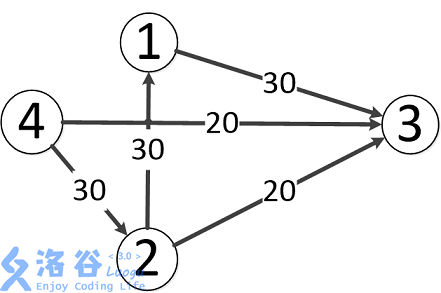
\includegraphics[width=0.5\textwidth]{images/flow1.png} 

\end{figure}

我们从 $4$ 到 $3$,肯定可以先从流量为 $20$ 的这条边先走。那么这条边就被走掉了,不能再选,总的流量为$20$(现在)。然后我们可以这样选择:

\begin{enumerate}
\item $4\rightarrow2\rightarrow3$ 这条\textbf{增广路}的总流量为 $20$。到 $2$ 的时候还是 $30$,到 $3$ 了就只有 $20$ 了。
\item $4\rightarrow2\rightarrow1\rightarrow3$ 这样子我们就很好的保留了 $30$ 的流量。
\end{enumerate}

所以我们这张图的最大流就应该是 $20+30=50$。

求最大流是很简单的,稍后我们会讲解求最大流的 $3$ 种方法。

\subsubsection{最小费用最大流 (MCMF)}

这也是耳熟能闻的费用流——最小费用最大流 (Minimum cost Maximum flow)。我们给予这张图一个费用值(也就是最短路问题),然后在求出最大流的基础上,把最小费用的路径求出来。这个难度就上升到了提高组的难度,并不是大家都可以先决的。

\subsubsection{最大流解法锦集}

所有代码请看:\href{https://www.luogu.org/paste/6t8jgtxc}{剪贴板}。

\paragraph{Edmond-Karp 动能算法($EK$ 算法)}

这个算法很简单,就是 DFS\textbf{找增广路},然后对其进行\textbf{增广}。你可能会问,怎么找?怎么增广?

\begin{enumerate}
\item 找? 我们就从源点一直 DFS 走来走去,碰到汇点就停,然后增广(每一条路都要增广)。我们在 DFS 的时候就注意一下流量合不合法就可以了。
\item 增广?其实就是按照我们找的增广路在重新走一遍。走的时候把这条路的能够成的最大流量减一减,然后给答案加上最小流量就可以了。
\end{enumerate}

再讲一下\textbf{反向边}。增广的时候要注意建造反向边,原因是这条路不一定是最优的,这样子程序可以进行反悔。假如我们对这条路进行增广了,那么其中的每一条边的反向边的流量就是它的流量。

\begin{figure}[h]
\centering
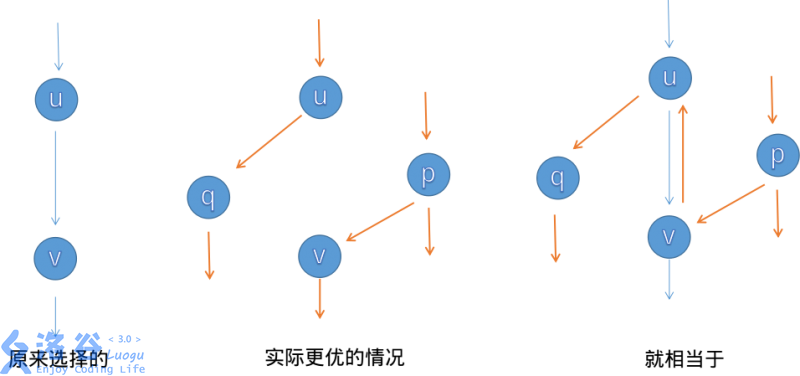
\includegraphics[width=0.5\textwidth]{images/flow2.png} 

\end{figure}

讲一下一些小细节。如果你是用邻接矩阵的话,反向边直接就是从 $table[x,y]$ 变成 $table[y,x]$。如果是常用的链式前向星,那么在加入边的时候就要先加入反向边。那么在用的时候呢,我们直接 $i\operatorname{xor}1$ 就可以了 ($i$ 为边的编号)。为什么呢? 相信大家都是知道 $\operatorname{xor}$ 的,那么我们在加入正向边后加入反向边,就是靠近的,所以可以使用 $\operatorname{xor}$。我们还要注意一开始的编号要设置为 $tot=1$,因为边要从编号 $2$ 开始,这样子 $\operatorname{xor}$ 对编号 $2,3$ 的边才有效果。

\subsubsection{Dinic}

我们知道,一条路一条路找是十分的慢的,我们就设想可不可以很多条路一起找。答案当然是可以的。我们只需要一个问题,这些路是同时找的,如果有些路很调皮,往回 (别的路) 找,那么别的路不就是异常尴尬。

我们给这张图每一条边都指定一个方向,就不会出现上述情况。这时候我们就可以知道 \textbf{分层} 这个概念。我们对于每一次增广以后的图,给它进行分层。我们规定,低的级别只能去高的级别的点(而且只能高 $1$ 级别)。而级别就是它与源点的距离。我们对于每一次整体增广来一次 BFS 就可以了。

\subsubsection{ISAP}

这个是 $SAP$ 算法的加强版 (Improved)。

\subsubsection{最小费用最大流解法}

最简单的就是 EK+SPFA,也推荐用 zkw 费用流和原始对偶匹配算法。

\subsubsection{网络流基础知识拓展}

前面都看懂的同学可以看一下以下内容。

\subsubsection{最小割}

割其实就是删边的意思,当然最小割就是割掉 $X$ 条边来让 $S$ 跟 $T$ 不互通。我们要求 $X$ 条边加起来的流量综合最小。这就是最小割问题。

其中我们要认识一个定理: \textbf{最小割}=\textbf{最大流}

\subsubsection{二分图匹配}

匈牙利算法就是其中一个可撤回贪心的过程,而网络流更快,就在于 \textbf{撤回} 这一过程很快。

\subsubsection{建模}

在会了最大流和费用流后,建模显得尤为重要。就像 JZOI 的 \href{https://www.luogu.org/problemnew/show/P2598}{狼与羊的故事},就是一个例子。

\textbf{前期}遇到这种题目,暴搜?神奇 BFS?错误。我们首先要考虑一下会不会有\textbf{二分图匹配},\textbf{最小割}的模型(一般不会有普通的最大流)。然后建立(超级)源点和(超级)汇点。什么意思?就是当很多个源点和很多个汇点的时候,我们就可以用超级源点和超级汇点代替「源点」和「汇点」的位置(也就是把超级源点连向各个源点,超级汇点连向各个汇点,方向按题意来定)。

这是最常见的建模的方法之一,也是做二分图匹配的方法。还有很多建模方法,可以参考 \href{https://www.cnblogs.com/victorique/p/8560656.html}{网络流建模基础}。

来一道题练练手: \href{https://www.luogu.org/paste/z3085b8l}{沙耶的玩偶}。
